\documentclass[aspectratio=43]{beamer}
%% \documentclass[aspectratio=169]{beamer}
\usetheme[
  block=fill,
  background=light,
  titleformat=smallcaps,
  progressbar=frametitle,
  numbering=none,
]{metropolis}
\setbeamersize{text margin left=.7cm,text margin right=.7cm}
\usepackage{appendixnumberbeamer}

%%%%%%%%%%%%%%%%%%%%%%%%%%%%%%%%%%%%%%%%%%
%% Packages
%%%%%%%%%%%%%%%%%%%%%%%%%%%%%%%%%%%%%%%%%%

% Tikz
\usepackage{tikz}
\usetikzlibrary{arrows,positioning,matrix,fit,backgrounds,decorations.text,decorations.pathmorphing,calc,shapes}

% Colors
\usepackage{xcolor}
\usepackage{contour}

% Images
\usepackage{graphics}
\graphicspath{{img/}}
\usepackage{caption}

% Math
\usepackage{amssymb}
\usepackage{stmaryrd}
\usepackage{proof}
\newenvironment{proposition}[1]
  {\begin{alertblock}{#1}\begin{displaymath}}
  {\end{displaymath}\end{alertblock}}

\newcommand\ADA[0]{\raisebox{-.25\height}{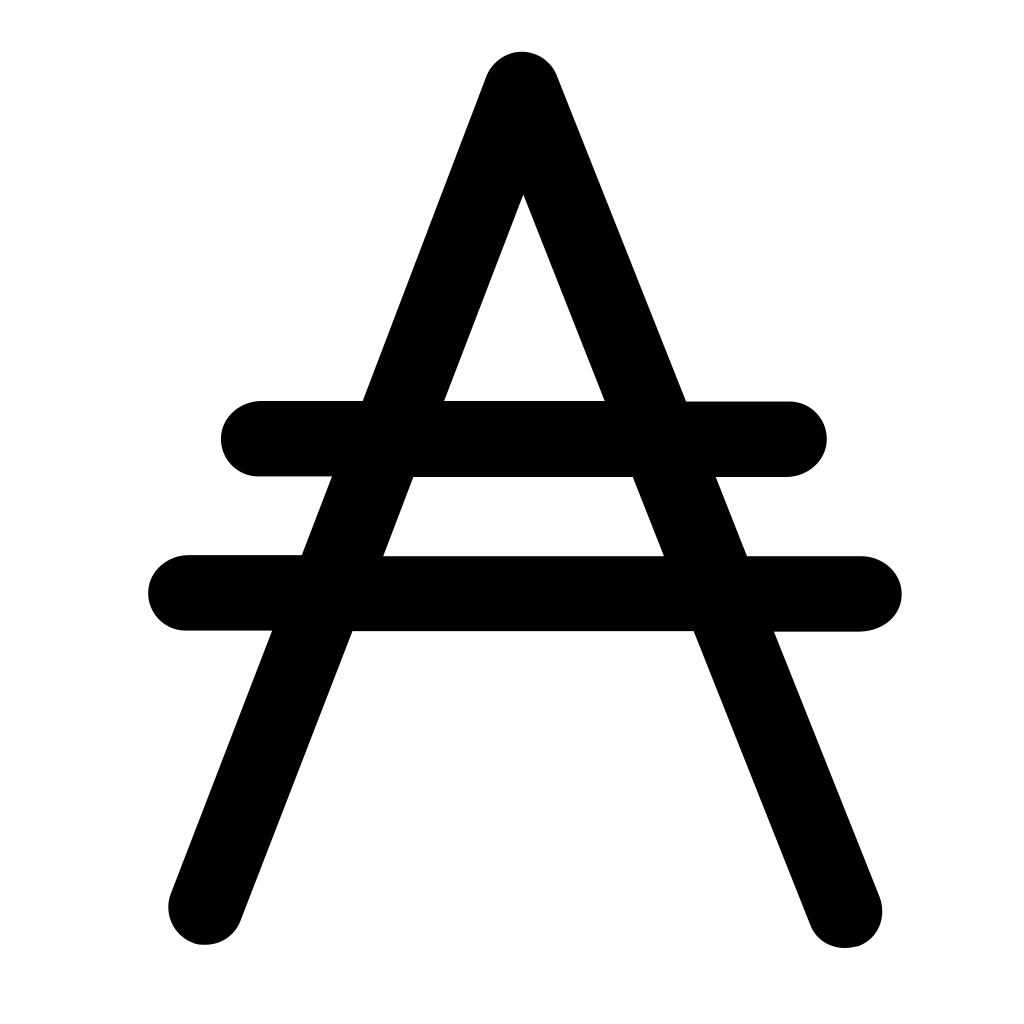
\includegraphics[keepaspectratio=true,height=10pt]{ada}}}


%%%%%%%%%%%%%%%%%%%%%%%%%%%%%%%%%%%%%%%%%%
%% Macros
%%%%%%%%%%%%%%%%%%%%%%%%%%%%%%%%%%%%%%%%%%
\renewcommand\alert[1]{\textcolor{mLightBrown}{#1}}
\newcommand\todo[1]{\textcolor{red}{#1}}

%% Counters for `enumerate`
\newcounter{saveenumi}
\newcommand{\seti}{\setcounter{saveenumi}{\value{enumi}}}
\newcommand{\conti}{\setcounter{enumi}{\value{saveenumi}}}

\renewcommand{\i}{\textit}  % Just to speed up typing: replace these in the final version
\renewcommand{\t}{\texttt}  % Just to speed up typing: replace these in the final version
\newcommand{\s}{\textsf}  % Just to speed up typing: replace these in the final version
\newcommand{\msf}[1]{\ensuremath{\mathsf{#1}}}
\newcommand{\mi}[1]{\ensuremath{\mathit{#1}}}

%% A figure with rules above and below.
\newcommand\rfskip{7pt}
%\newenvironment{ruledfigure}[1]{\begin{figure}[#1]\hrule\vspace{\rfskip}}{\vspace{\rfskip}\hrule\end{figure}}
\newenvironment{ruledfigure}[1]{\begin{figure}[#1]}{\end{figure}}

%% Various text macros
\newcommand{\true}{\ensuremath{\mathsf{true}}} % \textsf becomes slanted in math mode
\newcommand{\false}{\ensuremath{\textsf{false}}}

\newcommand{\hash}[1]{\ensuremath{#1^{\#}}}

\newcommand{\List}[1]{\ensuremath{\s{List}[#1]}}
\newcommand{\Set}[1]{\ensuremath{\s{Set}[#1]}}
\newcommand{\FinSet}[1]{\ensuremath{\s{FinSet}[#1]}}
\newcommand{\Interval}[1]{\ensuremath{\s{Interval}[#1]}}
\newcommand{\FinSup}[2]{\ensuremath{\s{FinSup}[#1,\linebreak[0]#2]}}
% ^ \linebreak is to avoid a bad line break when we talk about finite
% maps.  We may be able to remove it in the final version.

\newcommand{\supp}{\msf{supp}}

\newcommand{\Script}{\ensuremath{\s{Script}}}
\newcommand{\scriptAddr}{\msf{scriptAddr}}
\newcommand{\ctx}{\ensuremath{\s{Context}}}
\newcommand{\vlctx}{\ensuremath{\s{ValidatorContext}}}
\newcommand{\mpsctx}{\ensuremath{\s{PolicyContext}}}
\newcommand{\toData}{\ensuremath{\s{toData}}}
\newcommand{\toTxData}{\ensuremath{\s{toTxData}}}
\newcommand{\fromData}{\msf{fromData}}

\newcommand{\mkContext}{\ensuremath{\s{mkContext}}}
\newcommand{\mkVlContext}{\ensuremath{\s{mkValidatorContext}}}
\newcommand{\mkMpsContext}{\ensuremath{\s{mkPolicyContext}}}

\newcommand{\applyScript}[1]{\ensuremath{\llbracket#1\rrbracket}}
\newcommand{\applyMPScript}[1]{\ensuremath{\llbracket#1\rrbracket}}

% Macros for eutxo things.
\newcommand{\tx}{\mi{tx}}
\newcommand{\TxId}{\ensuremath{\s{TxId}}}
\newcommand{\txId}{\msf{txId}}
\newcommand{\txrefid}{\mi{id}}
\newcommand{\Address}{\ensuremath{\s{Address}}}
\newcommand{\DataHash}{\ensuremath{\s{DataHash}}}
\newcommand{\hashData}{\msf{dataHash}}
\newcommand{\idx}{\mi{index}}
\newcommand{\inputs}{\mi{inputs}}
\newcommand{\outputs}{\mi{outputs}}
\newcommand{\forge}{\mi{forge}}
\newcommand{\forgeScripts}{\mi{forgeScripts}}
\newcommand{\sigs}{\mi{sigs}}
\newcommand{\fee}{\mi{fee}}
\newcommand{\addr}{\mi{addr}}
\newcommand{\val}{\mi{value}}  %% \value is already defined

\newcommand{\validator}{\mi{validator}}
\newcommand{\redeemer}{\mi{redeemer}}
\newcommand{\datum}{\mi{datum}}
\newcommand{\datumHash}{\mi{datumHash}}
\newcommand{\datumWits}{\mi{datumWitnesses}}
\newcommand{\Data}{\ensuremath{\s{Data}}}
\newcommand{\Input}{\ensuremath{\s{Input}}}
\newcommand{\Output}{\ensuremath{\s{Output}}}
\newcommand{\OutputRef}{\ensuremath{\s{OutputRef}}}
\newcommand{\Signature}{\ensuremath{\s{Signature}}}
\newcommand{\Ledger}{\ensuremath{\s{Ledger}}}

\newcommand{\outputref}{\mi{outputRef}}
\newcommand{\outputrefs}{\mi{outputRefs}}
\newcommand{\txin}{\mi{in}}
\newcommand{\id}{\mi{id}}
\newcommand{\lookupTx}{\msf{lookupTx}}
\newcommand{\getSpent}{\msf{getSpentOutput}}

\newcommand{\Tick}{\ensuremath{\s{Tick}}}
\newcommand{\currentTick}{\msf{currentTick}}
\newcommand{\spent}{\msf{spentOutputs}}
\newcommand{\unspent}{\msf{unspentOutputs}}
\newcommand{\txunspent}{\msf{unspentTxOutputs}}
\newcommand{\eutxotx}{\msf{Tx}}

\newcommand{\Quantity}{\ensuremath{\s{Quantity}}}
\newcommand{\Asset}{\ensuremath{\s{Asset}}}
\newcommand{\Policy}{\ensuremath{\s{Policy}}}
\newcommand{\Quantities}{\ensuremath{\s{Quantities}}}
\newcommand{\nativeCur}{\ensuremath{\mathrm{nativeC}}}
\newcommand{\nativeTok}{\ensuremath{\mathrm{nativeT}}}

\newcommand\B{\ensuremath{\mathbb{B}}}
\newcommand\N{\ensuremath{\mathbb{N}}}
\newcommand\Z{\ensuremath{\mathbb{Z}}}
\renewcommand\H{\ensuremath{\mathbb{H}}}
%% \H is usually the Hungarian double acute accent
\newcommand{\emptyBs}{\ensuremath{\emptyset}}

\newcommand{\emptymap}{\ensuremath{\{\}}}

\newcommand{\outRef}{\mi{out}_{\mi{ref}}}
\newcommand{\fps}{\mi{fps}}
\newcommand{\fpss}{\mi{fpss}}

\usepackage{etoolbox}

\newcommand{\Cardano}{Cardano}
\newcommand{\PlutusCore}{Plutus Core}
\newcommand{\GitUser}{omelkonian}

% Macros for formalisation
\newcommand\agdaRepo{https://github.com/omelkonian/formal-utxo/tree/2d32}
\newcommand\ra{\rightarrow}
\newcommand\nft{\ensuremath{\blacklozenge}}
\newcommand\NF{\s{NonFungible}}
\newcommand\Trace{\s{Trace}}
\newcommand\Provenance{\s{Provenance}}
\newcommand\provenance{\s{provenance}}
\newcommand\isFinal{\msf{isFinal}}
\newcommand\step{\msf{step}}
\newcommand\satisfies{\msf{satisfies}}
\newcommand\checkOutputs{\msf{checkOutputs}}
\newcommand\initial{\msf{initial}}
\newcommand\extract{\msf{extract}}

\newcommand\All{\msf{All}}
\newcommand\AllS{\msf{All}^\s{S}}

\newcommand\mkValidator[1]{\msf{validator}_#1}
\newcommand\mkPolicy[1]{\msf{policy}_#1}
\newcommand\valC{\mkValidator{\mathcal{C}}}
\newcommand\polC{\mkPolicy{\mathcal{C}}}

\newcommand\CStepArrow[3]{\ensuremath{
#1 \xrightarrow{\hspace{5pt} #2 \hspace{5pt}} (#1' , #3)
}}

\newcommand\txeq{tx^\equiv}
\newcommand\Sim[2]{\ensuremath{
#1 \sim #2
}}
\newcommand\CStep[1]{\ensuremath{
 #1 \xrightarrow{\hspace{5pt} i \hspace{5pt}} (#1' , \txeq)
%%\textsf{step}\, #1\, i \equiv \textsf{just}\, #1'
}}
\newcommand\LStep[2]{\ensuremath{
#1 \xrightarrow{\hspace{5pt} #2 \hspace{5pt}} #1'
}}
\newcommand\transTo{\ensuremath{
    \rightsquigarrow^*
}}
\newcommand\transToN{\ensuremath{
    \rightsquigarrow^{+}
}}

% multisig
\newcommand{\msc}{\mathrm{msc}}
\newcommand{\sig}{\mathit{sig}}
%\newcommand{\sigs}{\mathit{sigs}}
\newcommand{\auth}{\mathrm{auth}}
\newcommand{\Holding}{\msf{Holding}}
\newcommand{\Collecting}[4]{\msf{Collecting}(#1, #2, #3, #4)}
\newcommand{\Propose}[3]{\msf{Propose}(#1, #2, #3)}
\newcommand{\Add}[1]{\msf{Add}(#1)}
\newcommand{\Cancel}{\msf{Cancel}}
\newcommand{\Pay}{\msf{Pay}}

% Names, for consistency
\newcommand{\UTXO}{UTXO}
\newcommand{\EUTXO}{E\UTXO{}}
\newcommand{\ExUTXO}{Extended \UTXO{}}
\newcommand{\CEM}{CEM}
\newcommand{\UTXOma}{\UTXO$_{\textrm{ma}}$}
\newcommand{\EUTXOma}{\EUTXO$_{\textrm{ma}}$}

%%%%%%%%%%%%%%%%%%%%%%%%%%%%%%%%%%%%%%%%%%
%% Fonts
%%%%%%%%%%%%%%%%%%%%%%%%%%%%%%%%%%%%%%%%%%
\usepackage{relsize}
\usepackage[tt=false]{libertine}
\usepackage[libertine]{newtxmath}

%----------------------------------------------------------------------------

\title{Native Custom Tokens in The Extended UTXO Model}
%\subtitle{}
\author{
Manuel M.T. Chakravarty, James Chapman, Kenneth MacKenzie, \\
\textbf{Orestis Melkonian}, Jann M\"uller, Michael Peyton Jones, Polina Vinogradova, Philip Wadler \\[5pt]
}
\date{\textit{October 28, 2020}}
\titlegraphic{
\vspace*{6.5cm}

\includegraphics[keepaspectratio=true,height=1.0cm]{uoe}\\
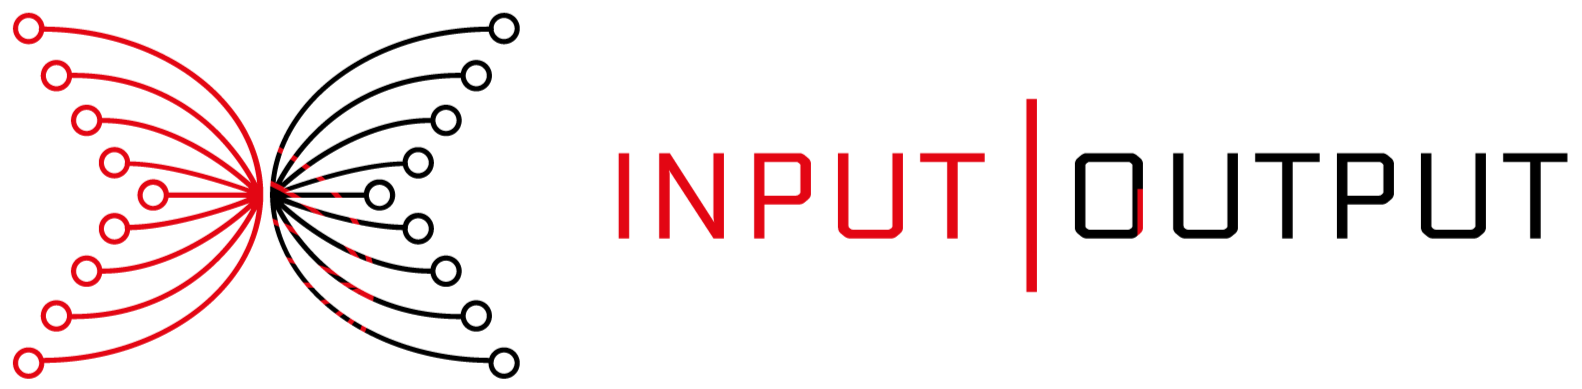
\includegraphics[keepaspectratio=true,height=0.8cm]{iohk}
}

\begin{document}
\begin{center}
\setbeamerfont{title}{size=\large}
\setbeamerfont{author}{size=\scriptsize}
\maketitle
\setbeamerfont{title}{size=\Large}
\end{center}

\tikzset{
  % global
  every matrix/.style =
  { ampersand replacement = \&,
    matrix of nodes,
    nodes in empty cells },
  % nodes
  boxx/.style = {align = center},
  box/.style =
  { %draw, rectangle,
    align          = center,
    minimum width  = .5cm,
    minimum height = 1.5cm },
  BG/.style =
  { rectangle,
    inner sep       = 0.2cm,
    rounded corners = 5mm,
    line width      = 1mm },
  MSc/.style =
  { BG, fill=yellow!25, text=yellow!25 },
  MSc-label/.style =
  { label={[name=msc]above left:\contour{yellow!25}{}} },
  PhD/.style =
  { BG, fill=orange!20, text=orange!20 },
  PhD-label/.style =
  { label={[name=phd]below:\contour{orange!20}{}} },
  PhD2/.style =
  { BG, fill=orange!30, text=orange!30 },
  PhD2-label/.style =
  { label={[name=phd]#1:\contour{orange!30}{}} },
  PhD3/.style =
  { BG, fill=green!25, text=green!25 },
  PhD3-label/.style =
  { label={[name=phd]#1:\contour{green!25}{}} },
  greenBox/.style =
  { BG, fill=green!15, },
%%   greenDot/.style =
%%   { BG , left color = red!35, middle color = green!55
%%   , bottom color = green!55, right color = green!55 },
  redDot/.style =
  { BG, draw=red!55, dashed },
  %% font=\small,
  txt/.style    = {align=center},
  note/.style   = {font=\small\itshape},
  accept/.style = {fill = green!15},
  reject/.style = {fill = red!15},
  cit/.style =
  { inner sep = 0.3cm, rounded corners = 2mm, font=\normalsize, align=center },
  % edges
  to/.style = {->, thick},
  squig/.style = {decorate, decoration={zigzag}}
}

\newcommand\bitml{
  \matrix (mat)
    [ column sep = 1.5cm,
      row sep = 2cm,
      every node/.style = txt
    ] {
    \node {\textbf{\underline{Syntax}}};
    \& \node (operA) {};
    \& \node (operB) {};
    \& \node {\textbf{\underline{Game-theoretic}}\\\textbf{\underline{Semantics}}}; \\[-1cm]
    \node (contracts) {BitML\\Contracts};
    \& \node (lts) {Small-step\\LTS};
    \& \node (sm) {Symbolic\\Runs};
    \& \node (ss) {Symbolic\\Strategies}; \\
    \node (transactions) {Bitcoin\\Transactions};
    \& \node (bc) {Blockchain\\Consistency};
    \& \node (cm) {Computational\\Runs};
    \& \node (cs) {Computational\\Strategies}; \\
  };
  \node[fit=(operA)(operB)]{\textbf{\underline{Operational Semantics}}};
  \path
  (contracts) edge[to]
    node[right] (comp) {$\mathcal{C}$}
  (transactions)
  (sm) edge[<->, bend left = 40]
    node[right] (coh) {$\sim$}
  (cm)
  (cm) edge[to]
    node[left] (parsing) {\textit{\alert{parse}}}
  (sm)
  (ss) edge[to]
    node[left] (n) {$\aleph$}
  (cs)
  (coh.east) edge[<->, double]
    node[above] (compsA) {\textit{\alert{computational}}}
    node[below] (compsB) {\textit{\alert{soundness}}}
  (n.west)
  (lts) edge[squig] (sm)
  (bc) edge[squig] (cm)
  ;
}

\newcommand\withLogo[2]{\raisebox{-.25\height}{\includegraphics[keepaspectratio=true,height=27pt]{#1}}~~#2}
\newcommand\no{\Large $\times$}
\newcommand\yes{\Large $\checkmark$}

\section{Introduction}
\begin{frame}[plain]


\renewcommand{\arraystretch}{2.5}
\begin{tabular}{l|l|c|c}
\textbf{\hfil\small Blockchain\hfil} & \textbf{\hfil\small Model\hfil} & \textbf{\small Turing-complete} & \textbf{\small Deterministic} \\
\hline
\withLogo{bitcoin}{Bitcoin} & UTXO & \no & \no \\
\hline
\hspace{3pt}\withLogo{ethereum}{\hspace{3pt}Ethereum} & Accounts & \yes & \no \\
\hline
\withLogo{ada}{Cardano (IOHK)} & EUTXO & \yes & \yes \\
\end{tabular}

\end{frame}

\begin{frame}{Methodology}
\begin{itemize}
\item Focus on validating the relevant meta-theory
  \begin{itemize}
  \item In contrast to validating individual contracts
  \end{itemize}
\item Fully mechanized approach, utilizing Agda's rich type system
\item Fits well with IOHK's research-oriented approach
\end{itemize}

\begin{tikzpicture}
  [basic box/.style = {
     draw,
     shape = rectangle,
     align = center,
     minimum width=2cm,
     minimum height=1.2cm,
     rounded corners},
   to/.style = {
     ->,
     >=stealth',
     semithick
  },
  every matrix/.style={column sep=.8cm, ampersand replacement=\&},
  font=\small
  ]
  \matrix{
     \node[basic box,draw=mLightBrown] (a) {pure\\ research};
  \& \node[basic box,draw=mLightBrown] (b) {mechanized\\ models};
  \& \node[basic box] (c) {reference\\ implementations};
  \& \node[basic box] (d) {production\\ code}; \\
  };

  \path
  (a) edge[to, mLightBrown] (b)
  (b) edge[to] (c)
  (c) edge[to] (d)
  ;
\end{tikzpicture}
\end{frame}

\begin{frame}[label=contributions]{Contributions}

\begin{itemize}
\setlength\itemsep{.25cm}

\item \textbf{Detailed description of the Extended UTXO model (EUTXO)}
\begin{center}
\scalebox{.7}{
  \begin{tikzpicture}
    \eutxo
  \end{tikzpicture}
}
\end{center}

\item \textbf{Formalization in} \raisebox{-.5\height}{
\includegraphics[height=.18\textheight]{agda}}\\

\item \textbf{Proof of bisimulation with a specific form of state machines}\\
\begin{center}
\scalebox{.6}{
  \begin{tikzpicture}
    \multisig
  \end{tikzpicture}
}
\end{center}

\end{itemize}

\end{frame}

\section{EUTXO}

\begin{frame}{UTXO vs EUTXO}
  \centering
  \begin{tikzpicture}
    \utxo
  \end{tikzpicture}
  \vspace{.5cm}
  \hfil\rule{.9\textwidth}{.4pt}\hfil
  \begin{tikzpicture}
    \eutxo
  \end{tikzpicture}
\end{frame}

% maybe add slides for data-values and contract-continuity

\begin{frame}{Running Example: Asynchronous Multi-signature Contract}
  \centering
  \begin{tikzpicture}
    \multisig
  \end{tikzpicture}

  \rule{.9\textwidth}{.4pt}

  Pay value $(v)$ to payee $(p)$ until deadline $(d)$
\end{frame}

\newcommand\multisigZoom{.9}
\begin{frame}<1>[label=multisig-eutxo,plain]
  \frametitle<2>{Limitation: Initial State}
  \only<2>{\renewcommand\multisigZoom{.7}}
  \centering

  \vspace{.5cm}
  \scalebox{\multisigZoom}{
    \begin{tikzpicture}
      \multisig
    \end{tikzpicture}
  }

  \vspace{-.5cm}
  \rule{.9\textwidth}{.4pt}

  \scalebox{.8}{\vbox{
    \begin{itemize}
      \item $\delta \in \{ \msf{Holding} , \msf{Collecting} \}$
      \item $\rho \in \{ \msf{Propose} , \msf{Add} , \msf{Cancel} , \msf{Pay} \}$
    \end{itemize}
    \vspace{-.5cm}
  }}

  \rule{.9\textwidth}{.4pt}

  \scalebox{.8}{
    \begin{tikzpicture}
      \eutxo
    \end{tikzpicture}
  }
\end{frame}

\begin{frame}{Previous Work~~[The Extended UTXO Model @ WTSC'20]}
  \begin{itemize}
  \setlength\itemsep{.25cm}

  \item \textbf{Detailed description of the Extended UTXO model (EUTXO)}
  \begin{center}
  \scalebox{.7}{
    \begin{tikzpicture}
      \eutxo
    \end{tikzpicture}
  }
  \end{center}

  \item \textbf{Formalization in} \raisebox{-.5\height}{
\includegraphics[height=.18\textheight]{agda}}\\

  \item \textbf{Proof of bisimulation with a Constraint Emitting Machines (CEMs)}\\
  \begin{center}
  \scalebox{.6}{
    \begin{tikzpicture}
      \multisig
    \end{tikzpicture}
  }
  \end{center}

  \end{itemize}
\end{frame}

\againframe<2>{multisig-eutxo} % talk about CEM limitation, initial states

\section{\EUTXOma}

\begin{frame}{Token Bundles}
  \[
  \{\ADA \mapsto \{\ADA \mapsto 3\}, WoW \mapsto \{sword \mapsto 1, shield \mapsto 1\}\}
  \]
\end{frame}

\begin{frame}{Operations on Token Bundles}
  \begin{align*}
  & \{\ADA \mapsto \{\ADA \mapsto 3\}, WoW \mapsto \{sword \mapsto 1, shield \mapsto 1\}\} \\
  + \ & \{\ADA \mapsto \{\ADA \mapsto 1\}, WoW \mapsto \{armour \mapsto 1\}\} \\
  = \ & \{\ADA \mapsto \{\ADA \mapsto 4\}, WoW \mapsto \{sword \mapsto 1, shield \mapsto 1, armour \mapsto 1\}\} \ .
  \end{align*}
\end{frame}

\begin{frame}{Forging}
  \begin{itemize}[<+->]
  \item $Tx = \{ \dots \forge : \msf{TokenBundle}, policies : \sigma \rightarrow \msf{Bool} \dots \}$
  \item $\forge \in \mathbb{Z}^+ $ for minting, $\forge \in \mathbb{Z}^-$ for burning
  \item $\forall\ p\sharp \in \forge.domain: p \in policies \land p(\sigma) = \msf{True}$
  \end{itemize}
\end{frame}

\begin{frame}{Applications}
  \begin{itemize}
  \item Tokenised roles
  \item Fairness in ICO setup
  \item Algorithmic stablecoins

  \hspace{1cm} $\vdots$
  \end{itemize}
\end{frame}

\begin{frame}{Applications: Threaded State Machines}
  \begin{itemize}[<+->]
  \item Every CEM instance is associated with a unique token $\nft$
  \item \textbf{CEM policy:} check $\nft$ is minted in an initial state
  \item \textbf{CEM validator:} check $\nft$ is propagated at each transition
  \item[] $\implies$ can distinguish between different executions
  \item[] $\implies$ solve the initialisation problem
  \end{itemize}
\end{frame}

\section{Meta-theory}

\begin{frame}{Token Provenance}
  \begin{itemize}
  \item $\s{Token} = \s{Policy} \times \s{Asset}$
  \pause
  \item $\Trace(l,o,\nft,n) = t_0,\dots, t_i, t_{i+1},\dots, t_k$, where
    \begin{enumerate}
    \item $t_0.\forge^\nft \geq n$
    \item $t_i \overset{\nft}{\longrightarrow} t_{i+1} \geq n$
    \item $o \in t_k.\outputs$
    \end{enumerate}
  \pause
  \item $\Provenance(l,o,\nft) = \dots \Trace(l,o,\nft, n_i) \dots$ s.t. $\sum n_i \ge o.\val^\nft$
  \end{itemize}

  \pause

  \begin{proposition}{Every output has a provenance}
  \infer[\textsc{Provenance}]
    {\provenance(l,o,\nft) : \Provenance(l,o,\nft)}
    {o \in \{ t.\outputs \ | \ t \in l \}}
  \end{proposition}
\end{frame}

\begin{frame}{Example Traces}
  \centering
  \scalebox{.7}{
    \begin{tikzpicture}
      \traces
      \begin{pgfonlayer}{background}
        \onslide<+->{\node [Trace, fit=(j)] {};}

        \onslide<+-6>{\node [Trace, fit=(j)(i)] {};}
        \onslide<+-6>{\node [TraceNF, fit=(i)(h)] {};}
        \onslide<+-6>{\node [TraceNF, fit=(h)(g)] {};}
        \onslide<+-6>{\node [TraceNF, fit=(g)(f)] {};}
        \onslide<+>{\node [TraceNF, fit=(f)(e)] {};}

        \onslide<+-11>{\node [Trace, fit=(j)(i)] {};}
        \onslide<+-11>{\node [TraceFF, fit=(i)(d)] {};}
        \onslide<+-11>{\node [TraceFF, fit=(d)(c)] {};}
        \onslide<+-11>{\node [TraceFF, fit=(c)(b)] {};}
        \onslide<+>{\node [TraceFF, fit=(b)(a)] {};}

        \onslide<+->{\node [Trace, fit=(j)(i)] {};}
        \onslide<+->{\node [TraceFU, fit=(i)(d)] {}; \node [TraceF, fit=(i)(h)] {};}
        \onslide<+->{\node [TraceFU, fit=(d)(c)] {}; \node [TraceF, fit=(h)(g)] {};}
        \onslide<+->{\node [TraceFU, fit=(c)(b)] {}; \node [TraceF, fit=(g)(f)] {};}
        \onslide<+->{\node [TraceFU, fit=(b)(a)] {}; \node [TraceF, fit=(f)(e)] {};}
      \end{pgfonlayer}
    \end{tikzpicture}
  }
\end{frame}

\begin{frame}{Forging Policies}
  \begin{proposition}{Provenance is never empty}
  \infer[\textsc{Provenance}^+]
    {|\provenance(l, o, \nft)| > 0}
    {%
      o \in \{ t.\outputs \ | \ t \in l \}
    & o.\val^\nft > 0
    }
  \end{proposition}
  \pause
  \vspace{1cm}
  \begin{proposition}{Global Preservation}
  \sum_{t \in l} t.\forge = \sum_{o \in \unspent(l)} o.\val
  \end{proposition}
\end{frame}

\begin{frame}{Non-fungible Provenance}
  \begin{proposition}{Provenance for non-fungible tokens}
  \infer[\textsc{NF-Provenance}]
    {|\provenance(l, o, \nft)| = 1}
    {%
      o \in \{ t.\outputs \ | \ t \in l \}
    & o.\val^\nft > 0
    & \sum_{t \in l} t.\forge^\nft \leq 1
    }
  \end{proposition}
\end{frame}

\begin{frame}{Threaded CEMs}
  \begin{displaymath}
  \polC(\mi{txInfo}, c) = \left\{
    \begin{array}{lll}
    \true  & \mi{if} \ \mi{txInfo}.\forge^\nft = 1 \\
           & \mi{and} \ \s{origin} \in \mi{txInfo}.\outputrefs \\
           & \mi{and} \ \initial(\mi{txInfo}.\mi{outputs}^\nft) \\
    \false & \mi{otherwise}
    \end{array}
  \right.
  \end{displaymath}
  \pause
  \begin{displaymath}
  \color{gray}
  \valC(s, i, \mi{txInfo}) = \left\{
    \begin{array}{ll}
    \true  & \mi{if}  \ \CStep{s} \\
           & \mi{and} \ \satisfies(\mi{txInfo}, \txeq) \\
           & \mi{and} \ \checkOutputs(s', \mi{txInfo}) \\
           & \begingroup\color{black}
             \mi{and} \ \s{propagates}(\mi{txInfo}, \nft, s, s')
             \endgroup \\
    \false & \mi{otherwise}
    \end{array}
  \right.
  \end{displaymath}
\end{frame}

\begin{frame}{Threaded CEMs: Initiality}
  \begin{proposition}{All traces originate from initial states}
  \infer[\textsc{Initiality}]
    { \exists tr. \ \s{provenance}(l, o, \nft) = \{ tr \}
    \ \land \
      \polC(tr_0.\s{context}) = \true
    }
    {%
      o \in \{ t.\outputs \ | \ t \in l \}
    & o.\val^\nft > 0
    }
  \end{proposition}
\end{frame}

\begin{frame}{Property Preservation}
  \begin{proposition}{Well-rooted sequences}
  \infer[]
    {s \transTo s}
    {\initial(s) = \true}
  \qquad
  \infer[]
    {s \transTo s''}
    { s \transTo s'
    & \CStep{s'}
    }
  \end{proposition}
  \vspace{1cm}
  \pause
  \begin{proposition}{A property $P$ is invariant when:}
  \infer[]
    {\texttt{invariant}\ P}
    { \initial \implies P
    & \ \ \forall(s \transTo s'). P(s) \implies P(s')
    }
  \end{proposition}
\end{frame}

\begin{frame}{Example: Counter CEM}
  \begin{proposition}{}
  \begin{array}{l}
    (\mathbb {Z}, \{\mathsf{inc}\}, \step, \initial)\
    \mathbf{where}\
    \step(i,\mathsf{inc}) = \mathsf{just}(i + 1);\
    \initial(0) = \true
  \end{array}
  \end{proposition}
  \pause
  \begin{itemize}
  \item $Q = (\_ >= 0)$ is invariant, since $Q(0)$ and $Q(x) \implies Q(x + 1)$
  \end{itemize}
  \pause
  \begin{proposition}{Extracting CEM traces from EUTXO traces}
  \infer[\textsc{Extraction}]
    {tr.source \transTo tr.destination}
    {\provenance(l, o, \nft) = \{ tr \}}
  \end{proposition}
\end{frame}

\begin{frame}{Beyond Safety}
  \begin{itemize}
  \item so far only \alert{safety} properties
  \pause
  \item what about \alert{temporal} ones?
  \pause
    \begin{itemize}
    \item[] $\overset{?}{\implies}$ \textit{coinductive} techniques for \textit{infinitary} semantics
    \end{itemize}
  \end{itemize}
\end{frame}

\begin{frame}{Related Work}

\begin{itemize}
\item \alert{Bitcoin Covenants}~~[Möser et al. @ FC'16]
  \begin{itemize}
  \item Allows restricting how output values will be used in the future
  \item Major inspiration for our introduction of \textit{data values}
  \end{itemize}
\item \alert{Bitcoin Modelling Language (BitML)}~~[Bartoletti et al. @ CCS'18]
  \begin{itemize}
  \item Process-calculus with automata-based operational semantics
  \item Compiles down to standard Bitcoin transactions
  \item Quite complicated translation and requires off-chain communication
  \end{itemize}
\item \alert{Scilla}~~[Sergey et al. @ OOPSLA'19]
  \begin{itemize}
  \item For Ethereum-like contracts, using \textit{communicating automata}
  \item Embedded in Coq, allows proving temporal (hyper-)properties
  \end{itemize}
\item \alert{Timed Automata}~~[Andrychowicz et al. @ FORMATS'14]
  \begin{itemize}
  \item Pragmatic model checking of Bitcoin contracts using \textsc{UPPAAL}
  \item Does not come with formal guarantees though
  \end{itemize}
\end{itemize}

\end{frame}

\againframe{contributions}


\againframe{contributions}

\begin{frame}[standout]
  Questions?
\end{frame}

\end{document}
